%=============================================================%
\section{Kernel density estimaton}
\begin{frame}[fragile]
	
The kernel density estimate may be less familiar, but it can be a useful tool for plotting the shape of a distribution. Like the histogram, the KDE plots encodes the density of observations on one axis with height along the other axis:

sns.distplot(x, hist=False, rug=True);
\begin{figure}
	\centering
	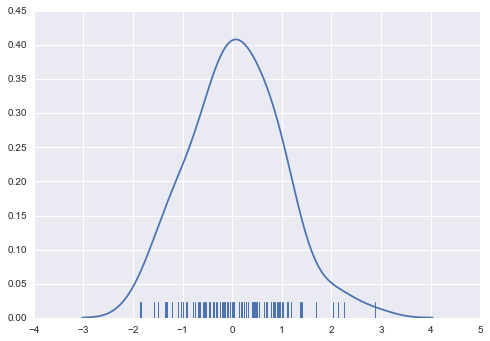
\includegraphics[width=0.7\linewidth]{images/distributions_14_0}
\end{figure}
\end{frame}
%============================================================%
\begin{frame}[fragile]
Drawing a KDE is more computationally involved than drawing a histogram. What happens is that each observation is first replaced with a normal (Gaussian) curve centered at that value:

\begin{frame}[fragile]
\begin{framed}
\begin{verbatim}

x = np.random.normal(0, 1, size=30)
bandwidth = 1.06 * x.std() * x.size ** (-1 / 5.)
support = np.linspace(-4, 4, 200)

kernels = []
for x_i in x:

    kernel = stats.norm(x_i, bandwidth).pdf(support)
    kernels.append(kernel)
    plt.plot(support, kernel, color="r")

\end{verbatim}
\end{framed}
\end{frame}
%=============================================================%
sns.rugplot(x, color=".2", linewidth=3);
\begin{figure}
	\centering
	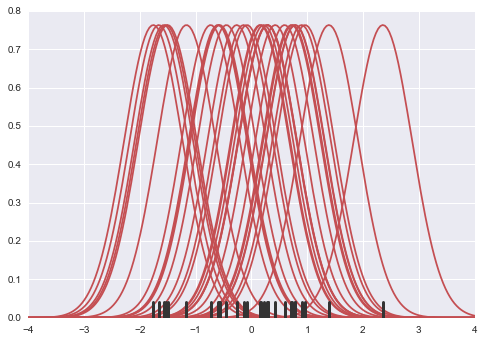
\includegraphics[width=0.7\linewidth]{images/distributions_16_0}
\end{figure}
Next, these curves are summed to compute the value of the density at each point in the support grid. The resulting curve is then normalized so that the area under it is equal to 1:

density = np.sum(kernels, axis=0)
density /= integrate.trapz(density, support)
plt.plot(support, density);
\begin{figure}
	\centering
	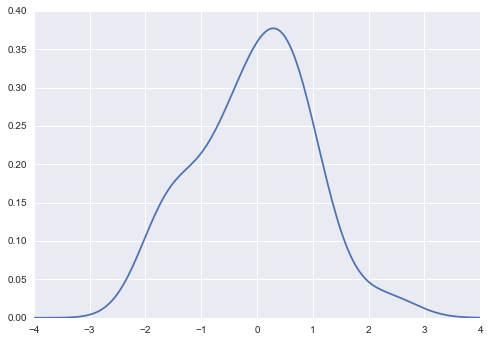
\includegraphics[width=0.7\linewidth]{images/distributions_18_0}
\end{figure}
\end{frame}
%===========================================================%
\begin{frame}
We can see that if we use the kdeplot() function in seaborn, we get the same curve. This function is used by distplot(), but it provides a more direct interface with easier access to other options when you just want the density estimate:

sns.kdeplot(x, shade=True);
../_images/distributions_20_0.png
\end{frame}
\begin{frame}
The bandwidth (bw) parameter of the KDE controls how tightly the estimation is fit to the data, much like the bin size in a histogram. It corresponds to the width of the kernels we plotted above. The default behavior tries to guess a good value using a common reference rule, but it may be helpful to try larger or smaller values:

sns.kdeplot(x)
sns.kdeplot(x, bw=.2, label="bw: 0.2")
sns.kdeplot(x, bw=2, label="bw: 2")
plt.legend();
\begin{figure}
\centering
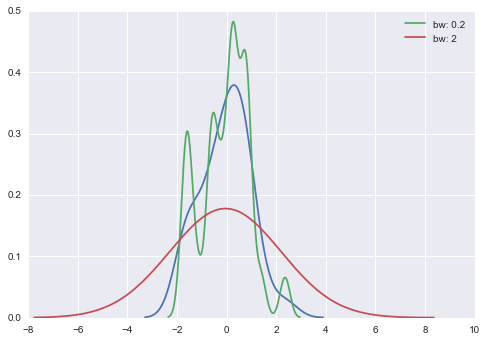
\includegraphics[width=0.7\linewidth]{images/distributions_22_0}
\caption{}
\label{fig:distributions_22_0}
\end{figure}

\end{frame}
%===========================================================%
\begin{frame}
	\large
As you can see above, the nature of the Gaussian KDE process means that estimation extends past the largest and smallest values in the dataset. It’s possible to control how far past the extreme values the curve is drawn with the cut parameter; however, this only influences how the curve is drawn and not how it is fit:

\begin{verbatim}
sns.kdeplot(x, shade=True, cut=0)
sns.rugplot(x);
\end{verbatim}
\end{frame}
%============================================================%
\begin{frame}[fragile]
\begin{figure}
\centering
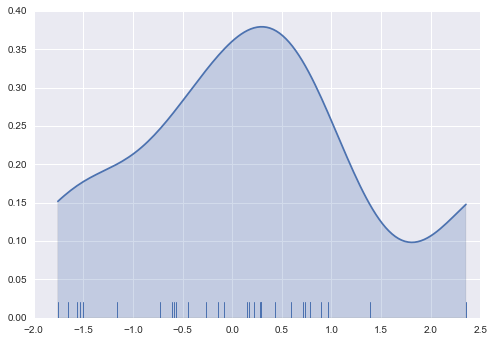
\includegraphics[width=0.7\linewidth]{images/distributions_24_0}
\caption{}
\label{fig:distributions_24_0}
\end{figure}
\end{frame}
\section{Fitting parametric distributions}
%============================================================%
\begin{frame}[fragile]
\noindent \textbf{Fitting parametric distributions}\\
You can also use distplot() to fit a parametric distribution to a dataset and visually evaluate how closely it corresponds to the observed data:
\begin{framed}
\begin{verbatim}
x = np.random.gamma(6, size=200)
sns.distplot(x, kde=False, fit=stats.gamma);
\end{verbatim}
\end{framed}

\end{frame}
%============================================================%
\begin{frame}[fragile]
\begin{figure}
\centering
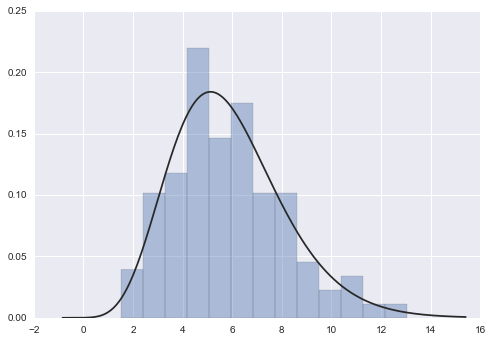
\includegraphics[width=0.7\linewidth]{images/distributions_26_0}
\caption{}
\label{fig:distributions_26_0}
\end{figure}


\end{document}